\section{Background: Complexity of Modeling Modern Manufacturing}
\label{sec::background}

%In this paper, we consider discrete manufacturing systems -- an important class
%of CPS that are in use today \cite{flex-reconf-2005}.
The physical part of a manufacturing system consists of machines and material handling devices (\eg robots and
conveyors). Machines and robots typically have their own low-level controllers (these are denoted MC and RC in Figure~\ref{fig::today}). Raw or unfinished parts arrive at the
system, are transported via material handling and exit the system in a
finished state. 
%
%The {\em cyber} side consists of a collection of controllers and communication networks. 
The system also has  multiple {\em Logic
Controllers} (LCs), often implemented on PLC hardware. These LCs read data
from sensors and send commands to actuators. LCs are typically local
controllers that coordinate a physical region of a plant, called a {\em cell}.
The LCs enable the production process by sending the right commands  to the
right actuators at the {\em right times}. Each LC is typically paired with a
{\em Safety Controller} (SC), a special type of logic controller that, instead
of enabling production, prohibits the manifestation of unsafe behavior in the
system. This is primarily for humans interacting with the physical system. For
instance, if an emergency-stop button is pressed then all of the machines,
robots and conveyors within the sphere of influence should stop as quickly (and
safely) as possible. In current practice, these LCs and SCs are individually programmed by
control engineers, using templates and style guidelines. Though these
controllers may operate for years or even decades due to exhaustive testing and
experienced design, this ``distributed'' style of programming  makes the
process of managing and reconfiguring such systems {\em difficult, error prone and even
insecure}. For the purposes of this paper, the MCs, RCs, LCs, SCs
and the various machines are all part of the `plant' while the `controler' is as
described in Section \ref{sec:intro} -- the centralized controler that oversees/manages 
the entire system. 

\begin{figure}[htb]
%\begin{wrapfigure}{r}{0.6\textwidth}
%\vspace{-\baselineskip}
\small
\centering
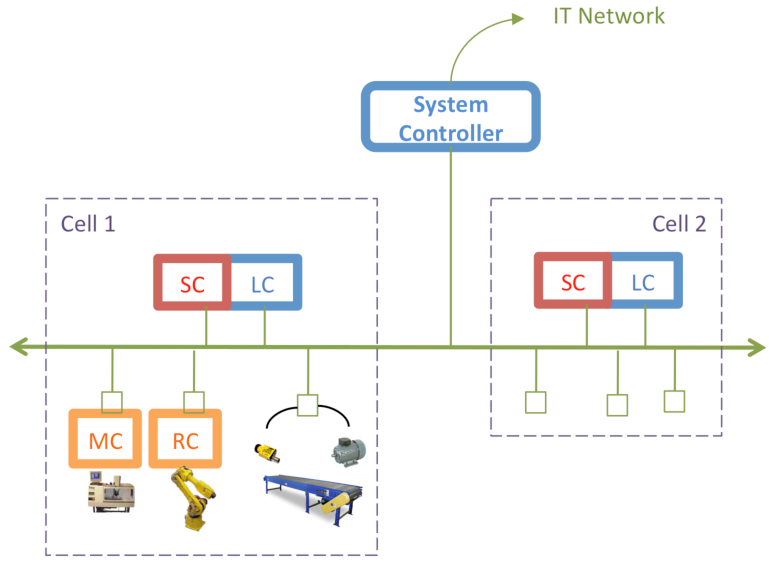
\includegraphics[width=0.95\columnwidth]{Figures/mfg-today.pdf}
\vspace{-\baselineskip}
\caption{Tomorrow's Manufacturing Control Systems.}%
\label{fig::today}
% \noindent \hrule
\vspace{-\baselineskip}
%\end{wrapfigure}
\end{figure}
